%%%%%%%%%%%%%%%%%%%%%%%%%%%%%%%%%%%%%%%%%%%%%%%%%%%%%%%%%%%%%%%%%%%%%%%%%%%%%%%%
% TUM-Vorlage: Präsentation
%%%%%%%%%%%%%%%%%%%%%%%%%%%%%%%%%%%%%%%%%%%%%%%%%%%%%%%%%%%%%%%%%%%%%%%%%%%%%%%%
%
% Rechteinhaber:
%     Technische Universität München
%     https://www.tum.de
% 
% Gestaltung:
%     ediundsepp Gestaltungsgesellschaft, München
%     http://www.ediundsepp.de
% 
% Technische Umsetzung:
%     eWorks GmbH, Frankfurt am Main
%     http://www.eworks.de
%
%%%%%%%%%%%%%%%%%%%%%%%%%%%%%%%%%%%%%%%%%%%%%%%%%%%%%%%%%%%%%%%%%%%%%%%%%%%%%%%%


%%%%%%%%%%%%%%%%%%%%%%%%%%%%%%%%%%%%%%%%%%%%%%%%%%%%%%%%%%%%%%%%%%%%%%%%%%%%%%%%
% Zur Wahl des Seitenverhältnisses bitte einen der beiden folgenden Befehle
% auskommentieren und den ausführen lassen:
% \documentclass[t]{beamer}
\usepackage[
    orientation=landscape,
    size=custom,
    width=25.4,
    height=19.05,
    scale=0.63 % erzeugt 16pt Schriftgröße
]{beamerposter}

\newcommand{\PraesentationSchriftgroesseSehrGross}{\fontsize{30}{45}}
\newcommand{\PraesentationSchriftgroesseGross}{\fontsize{22}{33}}
\newcommand{\PraesentationSchriftgroesseNormal}{\fontsize{16}{29}}
\newcommand{\PraesentationSchriftgroesseKlein}{\fontsize{12}{18}}
\newcommand{\PraesentationSchriftgroesseDreizeiler}{\fontsize{7}{10}}
\newcommand{\PraesentationSchriftgroesseAufzaehlungszeichen}{\fontsize{10}{8}}

\newcommand{\PraesentationAbstandAbsatz}{22.1pt}
\newcommand{\PraesentationPositionKorrekturOben}{0cm}
\newcommand{\PraesentationBeispieleSchriftgroessen}{30 | 22 | 16 | 12}
\documentclass[10pt]{scrlttr2} % Dokumentenklasse: KOMA-Skript Letter

% Anpassbare Kopf- und Fußzeilen für KOMA-Skript:
%\usepackage{scrlayer-scrpage}

\usepackage[utf8]{inputenc} % Textkodierung: UTF-8
\usepackage[T1]{fontenc} % Zeichensatzkodierung

\usepackage{calc} % Berechnungen

\usepackage[ngerman]{babel} % Deutsche Lokalisierung
\usepackage{graphicx} % Grafiken
\usepackage[absolute]{textpos} % Positionierung

% Silbentrennung:
\usepackage{hyphenat}
%\tolerance 2414
%\hbadness 2414
%\emergencystretch 1.5em
%\hfuzz 0.3pt
%\widowpenalty=10000     % Hurenkinder
%\clubpenalty=10000      % Schusterjungen
%\vfuzz \hfuzz

% Euro-Symbol:
\usepackage[gen]{eurosym}
\DeclareUnicodeCharacter{20AC}{\euro{}}

% Schriftart Helvetica:
\usepackage[scaled]{helvet}
\renewcommand{\familydefault}{\sfdefault}

\usepackage{mathptmx} % skalierbare Formelschriften
\usepackage{xstring} % Textmanipulation
\usepackage{xcolor} % Farbdefinitionen

\usepackage{bookmark} % Lesezeichen

\usepackage{etoolbox} % Toggle-Definitionen
\newtoggle{StellenausschreibungGrafikOpportunities}
\togglefalse{StellenausschreibungGrafikOpportunities}

% Unterdrückung layoutbedingter Warnungen
\usepackage[immediate]{silence}
\WarningFilter[layout]{latex}{Label(s) may have changed.} % Referenz auf letzte Seite



% Debugging:
%\DeactivateWarningFilters[layout] % Unterdrückte Warnungen einschalten
%\usepackage{layout} % Layout-Informationen
%\usepackage{printlen} % Längenwerte ausgeben
 % Seitenverhältnis 4:3
%\documentclass[aspectratio=169]{beamer}
\documentclass[t,aspectratio=169]{beamer}
\usepackage[
    orientation=landscape,
    size=custom,
    width=25.4,
    height=14.2875,
    scale=0.5
]{beamerposter}

\newcommand{\PraesentationSchriftgroesseSehrGross}{\fontsize{25}{38}}
\newcommand{\PraesentationSchriftgroesseGross}{\fontsize{18}{27}}
\newcommand{\PraesentationSchriftgroesseNormal}{\fontsize{14}{21}}
\newcommand{\PraesentationSchriftgroesseKlein}{\fontsize{11}{17}}
\newcommand{\PraesentationSchriftgroesseDreizeiler}{\fontsize{7}{10}}
\newcommand{\PraesentationSchriftgroesseAufzaehlungszeichen}{\fontsize{10}{8}}

\newcommand{\PraesentationAbstandAbsatz}{18pt}
\newcommand{\PraesentationPositionKorrekturOben}{-1cm}
\newcommand{\PraesentationBeispieleSchriftgroessen}{25 | 18 | 14 | 11}
\documentclass[10pt]{scrlttr2} % Dokumentenklasse: KOMA-Skript Letter

% Anpassbare Kopf- und Fußzeilen für KOMA-Skript:
%\usepackage{scrlayer-scrpage}

\usepackage[utf8]{inputenc} % Textkodierung: UTF-8
\usepackage[T1]{fontenc} % Zeichensatzkodierung

\usepackage{calc} % Berechnungen

\usepackage[ngerman]{babel} % Deutsche Lokalisierung
\usepackage{graphicx} % Grafiken
\usepackage[absolute]{textpos} % Positionierung

% Silbentrennung:
\usepackage{hyphenat}
%\tolerance 2414
%\hbadness 2414
%\emergencystretch 1.5em
%\hfuzz 0.3pt
%\widowpenalty=10000     % Hurenkinder
%\clubpenalty=10000      % Schusterjungen
%\vfuzz \hfuzz

% Euro-Symbol:
\usepackage[gen]{eurosym}
\DeclareUnicodeCharacter{20AC}{\euro{}}

% Schriftart Helvetica:
\usepackage[scaled]{helvet}
\renewcommand{\familydefault}{\sfdefault}

\usepackage{mathptmx} % skalierbare Formelschriften
\usepackage{xstring} % Textmanipulation
\usepackage{xcolor} % Farbdefinitionen

\usepackage{bookmark} % Lesezeichen

\usepackage{etoolbox} % Toggle-Definitionen
\newtoggle{StellenausschreibungGrafikOpportunities}
\togglefalse{StellenausschreibungGrafikOpportunities}

% Unterdrückung layoutbedingter Warnungen
\usepackage[immediate]{silence}
\WarningFilter[layout]{latex}{Label(s) may have changed.} % Referenz auf letzte Seite



% Debugging:
%\DeactivateWarningFilters[layout] % Unterdrückte Warnungen einschalten
%\usepackage{layout} % Layout-Informationen
%\usepackage{printlen} % Längenwerte ausgeben
 % Seitenverhältnis 16:9
%%%%%%%%%%%%%%%%%%%%%%%%%%%%%%%%%%%%%%%%%%%%%%%%%%%%%%%%%%%%%%%%%%%%%%%%%%%%%%%%


%%%%%%%%%%%%%%%%%%%%%%%%%%%%%%%%%%%%%%%%%%%%%%%%%%%%%%%%%%%%%%%%%%%%%%%%%%%%%%%%
%%%%%%%%%%%%%%%%%%%%%%%%%%%%%%%%%%%%%%%%%%%%%%%%%%%%%%%%%%%%%%%%%%%%%%%%%%%%%%%%
% TUM-Vorlage: Personenspezifische Informationen
%%%%%%%%%%%%%%%%%%%%%%%%%%%%%%%%%%%%%%%%%%%%%%%%%%%%%%%%%%%%%%%%%%%%%%%%%%%%%%%%
%
% Rechteinhaber:
%     Technische Universität München
%     https://www.tum.de
% 
% Gestaltung:
%     ediundsepp Gestaltungsgesellschaft, München
%     http://www.ediundsepp.de
% 
% Technische Umsetzung:
%     eWorks GmbH, Frankfurt am Main
%     http://www.eworks.de
%
%%%%%%%%%%%%%%%%%%%%%%%%%%%%%%%%%%%%%%%%%%%%%%%%%%%%%%%%%%%%%%%%%%%%%%%%%%%%%%%%

% Für die Person anpassen:

\newcommand{\PersonTitel}{Dr.~rer.~nat.}
\newcommand{\PersonVorname}{Mohanad Kandil,}
\newcommand{\PersonNachname}{Alexandros Stathakopoulos}
\newcommand{\PersonStadt}{@Ort@}
\newcommand{\PersonAdresse}{%
    @Adresse@\\%
    @Plz@~\PersonStadt%
}
\newcommand{\PersonTelefon}{@Telefon@}
\newcommand{\PersonFax}{@Fax@}
\newcommand{\PersonEmail}{@E-Mail@}
\newcommand{\PersonWebseite}{@Web@}

\newcommand{\FakultaetAnsprechpartner}{@Ansprechpartner@}
\newcommand{\LehrstuhlName}{@Lehrstuhlname@}

\newcommand{\EinstellungBankName}{Bayerische Landesbank}
\newcommand{\EinstellungBankIBAN}{DE10700500000000024866}
\newcommand{\EinstellungBankBIC}{BYLADEMM}
\newcommand{\EinstellungSteuernummer}{143/241/80037}
\newcommand{\EinstellungUmsatzsteuerIdentifikationsnummer}{DE811193231}

\hyphenation{} % eigene Silbentrennung                    % !!! DATEI ANPASSEN !!!
%%%%%%%%%%%%%%%%%%%%%%%%%%%%%%%%%%%%%%%%%%%%%%%%%%%%%%%%%%%%%%%%%%%%%%%%%%%%%%%%

\renewcommand{\PersonTitel}{}
\newcommand{\Datum}{\today}

\renewcommand{\PraesentationFusszeileZusatz}{}

\title{Checkmate with AI}
\subtitle{Mastering Strategy Through Reinforcement Learning}
\author{Alexandros Stathakopoulos, Mohanad Kandil}
\institute[]{\UniversitaetName}
\date[\Datum]{Heilbronn, 09. Dezember 2024}
\subject{}


%%%%%%%%%%%%%%%%%%%%%%%%%%%%%%%%%%%%%%%%%%%%%%%%%%%%%%%%%%%%%%%%%%%%%%%%%%%%%%%%
%%%%%%%%%%%%%%%%%%%%%%%%%%%%%%%%%%%%%%%%%%%%%%%%%%%%%%%%%%%%%%%%%%%%%%%%%%%%%%%%
% EINSTELLUNGEN
%%%%%%%%%%%%%%%%%%%%%%%%%%%%%%%%%%%%%%%%%%%%%%%%%%%%%%%%%%%%%%%%%%%%%%%%%%%%%%%%

% Allgemein:
\newcommand{\AllgemeinGestalter}{ediundsepp Gestaltungsgesellschaft}
\newcommand{\AllgemeinErsteller}{eWorks GmbH}

% Universität:
\newcommand{\UniversitaetName}{Technische Universität München}
\newcommand{\UniversitaetAbkuerzung}{TUM}
\newcommand{\UniversitaetWebseite}{www.tum.de}
\newcommand{\UniversitaetLogoBreite}{19mm}
\newcommand{\UniversitaetLogoHoehe}{1cm}

\newcommand{\UniversitaetAdresse}{%
    Arcisstraße~21\\%
    80333~München%
}

% Fakultät:
\newcommand{\FakultaetName}{@Fakultät@}




% Seitenränder:
\newcommand{\SeitenrandOben}{20mm}
\newcommand{\SeitenrandRechts}{20mm}
\newcommand{\SeitenrandLinks}{25mm}
\newcommand{\SeitenrandUnten}{10mm}

% Falzmarken:
\newcommand{\FalzmarkeOben}{87mm}
\newcommand{\FalzmarkeMitte}{148.5mm}
\newcommand{\FalzmarkeUnten}{192mm}
\newcommand{\FalzmarkeBreite}{2mm}
\newcommand{\FalzmarkeDicke}{0.3pt}
\newcommand{\FalzmarkePositionLinks}{7mm}


% Adressfeld:
\newcommand{\AdressfeldHoehe}{45mm}
\newcommand{\AdressfeldBreite}{85mm}
\newcommand{\AdressfeldAbsenderSchriftgroesse}{7.5pt}
\newcommand{\AdressfeldEmpfaengerSchriftgroesse}{11pt}
\newcommand{\AdressfeldEmpfaengerZeilenabstand}{15pt}

% Text:
\newcommand{\TextOben}{77.5mm}
\newcommand{\TextSchriftgroesse}{11pt}
\newcommand{\TextZeilenabstand}{15pt}

% Fusszeile:
\newcommand{\FusszeilePositionOben}{271mm}
\newcommand{\FusszeileBreite}{165mm}
\newcommand{\FusszeileHoehe}{16.5mm}
\newcommand{\FusszeileZwischenabstand}{2mm}
\newcommand{\FusszeileBreiteGross}{44mm}
\newcommand{\FusszeileBreiteKlein}{35.0mm}
\newcommand{\FusszeileSeitennummerAbstand}{7.7mm}
\newcommand{\FusszeileSchriftgroesse}{7.5pt}
\newcommand{\FusszeileZeilenabstand}{8pt}


%%%%%%%%%%%%%%%%%%%%%%%%%%%%%%%%%%%%%%%%%%%%%%%%%%%%%%%%%%%%%%%%%%%%%%%%%%%%%%%%
% DOKUMENT
%%%%%%%%%%%%%%%%%%%%%%%%%%%%%%%%%%%%%%%%%%%%%%%%%%%%%%%%%%%%%%%%%%%%%%%%%%%%%%%%

\usepackage[a4paper,
    top=\SeitenrandOben,
    bottom=\SeitenrandUnten,
    inner=\SeitenrandLinks,
    outer=\SeitenrandRechts,
    foot=\FusszeileHoehe - 1mm,
    head=35mm,
    includefoot
]{geometry}

\textblockorigin{\SeitenrandLinks}{\SeitenrandOben} % Ursprung für Positionierung

% PDF-Einstellungen:
\usepackage{hyperref}
\hypersetup{
    hidelinks,
    pdfauthor={\PersonVorname{} \PersonNachname},
    pdftitle={\Betreff},
    pdfproducer={\AllgemeinErsteller},
    pdfcreator={\AllgemeinGestalter}
}

\renewcommand*{\raggedsignature}{\raggedright}

\makeatletter
    \@setplength{bfoldmarklength}{\FalzmarkeBreite}
    \@setplength{bfoldmarkvpos}{\FalzmarkeUnten}
    \@setplength{firstfoothpos}{\SeitenrandLinks - 2pt}
    \@setplength{firstfootvpos}{\FusszeilePositionOben}
    \@setplength{firstfootwidth}{\FusszeileBreite}
    \@setplength{foldmarkhpos}{\FalzmarkePositionLinks}
    \@setplength{foldmarkthickness}{\FalzmarkeDicke}
    \@setplength{mfoldmarklength}{\FalzmarkeBreite}
    \@setplength{mfoldmarkvpos}{\FalzmarkeMitte}

    \@setplength{refaftervskip}{\TextZeilenabstand}
    \@setplength{refvpos}{\TextOben}
    \@setplength{sigbeforevskip}{\baselineskip}
    \@setplength{sigindent}{0mm}
    \@setplength{subjectaftervskip}{\baselineskip + \baselineskip + 1pt}

    \@setplength{tfoldmarklength}{\FalzmarkeBreite}
    \@setplength{tfoldmarkvpos}{\FalzmarkeOben}
\makeatother

\KOMAoptions{
    fontsize=\TextSchriftgroesse,
    foldmarks=BMpTv,
    firsthead=false,
    backaddress=no,
    addrfield=no,
    fromalign=false
}

\setkomavar{fromname}{\UniversitaetName}
\setkomavar{fromaddress}{\PersonAdresse}
\addtokomafont{backaddress}{\fontsize{\AdressfeldAbsenderSchriftgroesse}{\AdressfeldAbsenderSchriftgroesse}\selectfont}
\addtokomafont{toaddress}{\fontsize{\AdressfeldEmpfaengerSchriftgroesse}{\AdressfeldEmpfaengerZeilenabstand}\selectfont}

\newcommand{\RuecksendeadresseTrenner}{~| \ignorespaces}

\AtBeginLetter{%
    % Logo:
    \begin{textblock*}{\UniversitaetLogoBreite}[1,0](\textwidth, 0cm)%
        \raggedleft%
        
\includegraphics{./Ressourcen/_Bilder/Universitaet_Logo_RGB.pdf}%
    \end{textblock*}%
    \setlength{\baselineskip}{\TextZeilenabstand}%
    \setlength{\parindent}{0mm} % keine Einrückung am Absatzanfang
    \setlength{\parskip}{\baselineskip} % einzeiliger Abstand nach Absätzen
    % Empfängerfenster:
    \begin{textblock*}{\AdressfeldBreite}[0,0](0cm, 15mm)%
        \raggedbottom\raggedright
        \begin{spacing}{.85}%
        {
            \usekomafont{backaddress}%
            \let\\\RuecksendeadresseTrenner% Umdefinieren von "\\" zu "~| "
            \Absender%
        } \\
        \end{spacing}
        \vspace*{5.5pt}
        \usekomafont{toaddress}%
        \EmpfaengerAdresse
    \end{textblock*}
}

\KOMAoptions{refline=dateleft}
\setkomavar{date}{\Datum}
\setkomavar{place}{\PersonStadt}
\setkomafont{subject}{\bfseries}
\setkomavar{subject}{\Betreff}
\setkomavar{signature}{\PersonVorname~\PersonNachname}

%\setkomavar*{enclseparator}{Anlage\vspace{-3em}}

\renewcommand*{\closing}[1]{#1\vspace*{3\baselineskip}\newline\usekomavar{signature}\newline}
\setkomavar{enclseparator}[Anlage]{~}
\renewcommand{\encl}[1]{\newline{}Anlage~#1}

\KOMAoptions{firstfoot=true}
\setkomafont{pagefoot}{\sffamily\fontsize{7.5pt}{8pt}\selectfont}
\renewcommand{\pagemark}{%
\begin{textblock*}{3em}[1,1](\paperwidth - \SeitenrandLinks - \SeitenrandRechts + \FusszeileSeitennummerAbstand + 3mm, \paperheight - \SeitenrandOben - \SeitenrandUnten)%
    \raggedleft\hfill\usekomafont{pagefoot}\thepage\,/\,\pageref*{LastPage}%
\end{textblock*}%
}

\setkomavar{firstfoot}{
    \TabPositions{2em}%
    \begin{minipage}[t][\FusszeileHoehe][t]{\FusszeileBreiteGross}%
        \usekomafont{pagefoot}%
        \textbf{\UniversitaetName}%
        \newline%
        \FakultaetName%
        \newline%
        \LehrstuhlName%
    \end{minipage}%
    \hspace*{\FusszeileZwischenabstand}%
    \begin{minipage}[t][\FusszeileHoehe][t]{\FusszeileBreiteGross}%
        \raggedright\usekomafont{pagefoot}%
        \textbf{\FakultaetAnsprechpartner}\newline%
        \PersonAdresse%
    \end{minipage}%
    \hspace*{\FusszeileZwischenabstand}%
    \begin{minipage}[t][\FusszeileHoehe][t]{\FusszeileBreiteKlein}%
        \raggedright\usekomafont{pagefoot}%
        Tel.\tab{\PersonTelefon}%
        \def\temp{\PersonFax}\ifx\temp\empty%
        \else%
          \newline Fax\tab{\PersonFax}%
        \fi%
        \newline\newline%
        \PersonEmail\newline%
        \href{http://\PersonWebseite}{\PersonWebseite}\newline%
        \href{http://\UniversitaetWebseite}{\UniversitaetWebseite}%
    \end{minipage}%
    \hspace*{\FusszeileZwischenabstand}%
    \begin{minipage}[t][\FusszeileHoehe][t]{\FusszeileBreiteKlein}%
        \raggedright\usekomafont{pagefoot}%
        \EinstellungBankName\newline%
        IBAN-Nr.: \EinstellungBankIBAN\newline%
        BIC: \EinstellungBankBIC\newline%
        Steuer-Nr.: \EinstellungSteuernummer\newline%
        USt-IdNr.: \EinstellungUmsatzsteuerIdentifikationsnummer\newline%
    \end{minipage}%
    \pagemark%
}

\begin{document}
\raggedright
\begin{letter}{}
\opening{\Gruss}

 % !!! NICHT ENTFERNEN !!!
%%%%%%%%%%%%%%%%%%%%%%%%%%%%%%%%%%%%%%%%%%%%%%%%%%%%%%%%%%%%%%%%%%%%%%%%%%%%%%%%

\graphicspath{ {Ressourcen/_Bilder/} }
%%%%%%%%%%%%%%%%%%%%%%%%%%%%%%%%%%%%%%%%%%%%%%%%%%%%%%%%%%%%%%%%%%%%%%%%%%%%%%%%
% FOLIENSTIL: Standard
\PraesentationMasterStandard

\PraesentationTitelseite % Fügt die Startseite ein

\begin{frame}
	\frametitle{Agenda}
	\vspace{0.5cm}
	\begin{enumerate}
		\item Historical Background
		\item Introduction to RL
		\item Introduction to Deep Q-Learning
		\item Discussion of Algorithms
		\item Project Planning
	\end{enumerate}
\end{frame}


\begin{frame}
	\frametitle{Historical Background}
	\vspace{0.5cm}
	Historical Progression
	\vspace{-0.2cm}
	\begin{itemize}
		\item Rooted in trial-and-error learning (Thorndike's Law of Effect)
		\item Incorporates dynamic programming and Markov Decision Processes
	\end{itemize}
	Advance in Games
	\vspace{-0.2cm}
	\begin{itemize}
		\item \textbf{Samuel's Checkers Player (1959)}: Demonstrated RL in game strategies 
				\begin{itemize}
					\item Used a value function for state evaluation
					\item Pioneered the use of \textbf{minimax strategy} combined with RL concepts
				\end{itemize}
		\item\textbf{ TD-Gammon (1992)}: Combined RL with neural networks for complex games (e.g., backgammon)
	\end{itemize}
\end{frame}

\begin{frame}
	\frametitle{Introduction}
	\vspace{1cm}
	\centering
	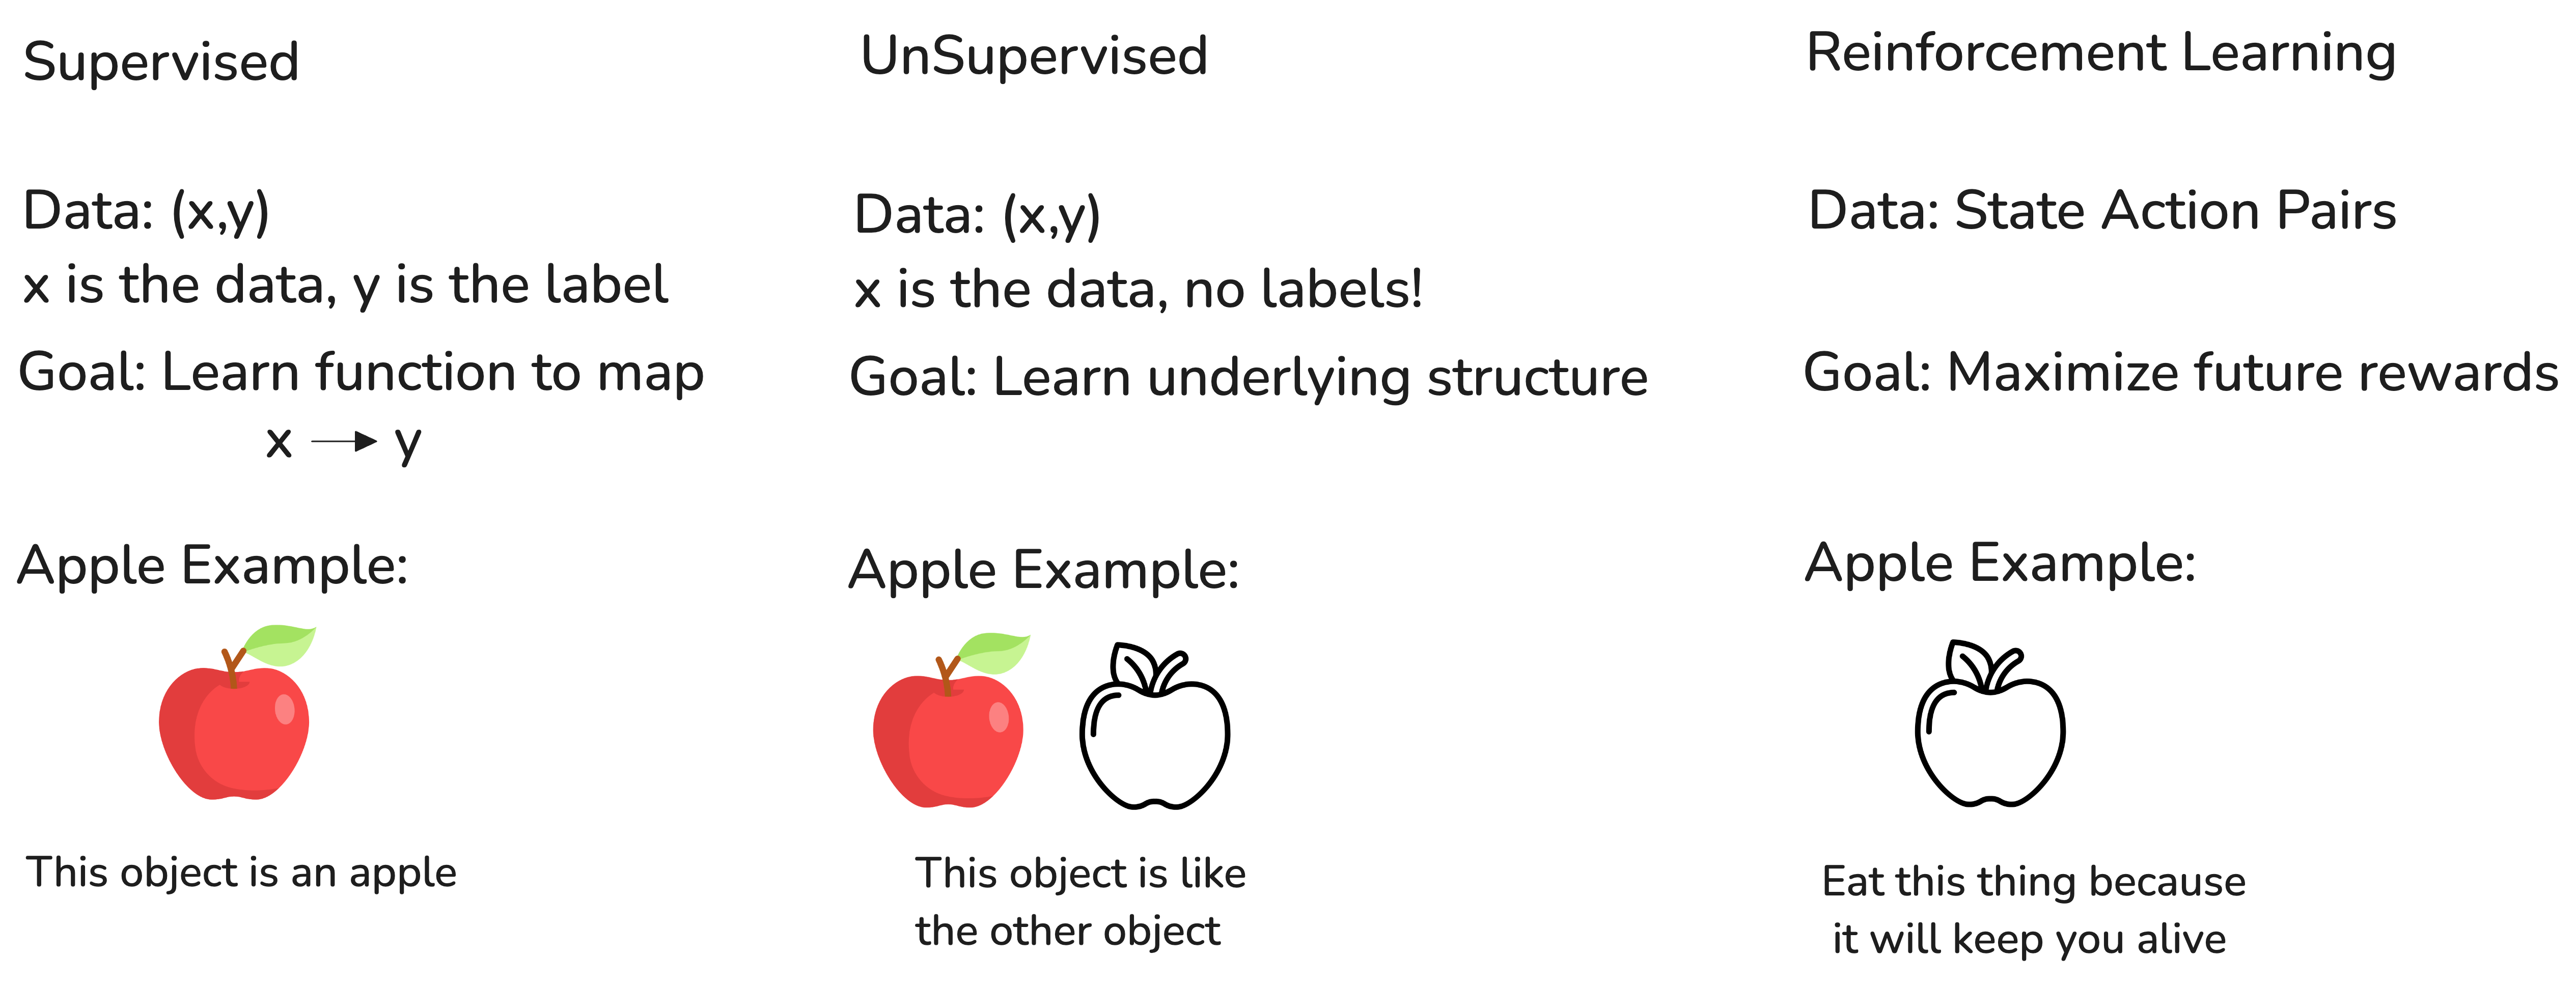
\includegraphics[scale=0.1]{appleNYC}
\end{frame}

\begin{frame}
	\frametitle{Introduction}
	\vspace{0.5cm}
	\begin{itemize}
		\item Checkers is a strategy game involving diagonal moves of pieces and captures by jumping over opponent pieces
		\item The objective of the project is to create an AI player using reinforcement learning
		\item Techniques: Q-learning and Deep Q-Networks (DQN)
	\end{itemize}
	\centering
	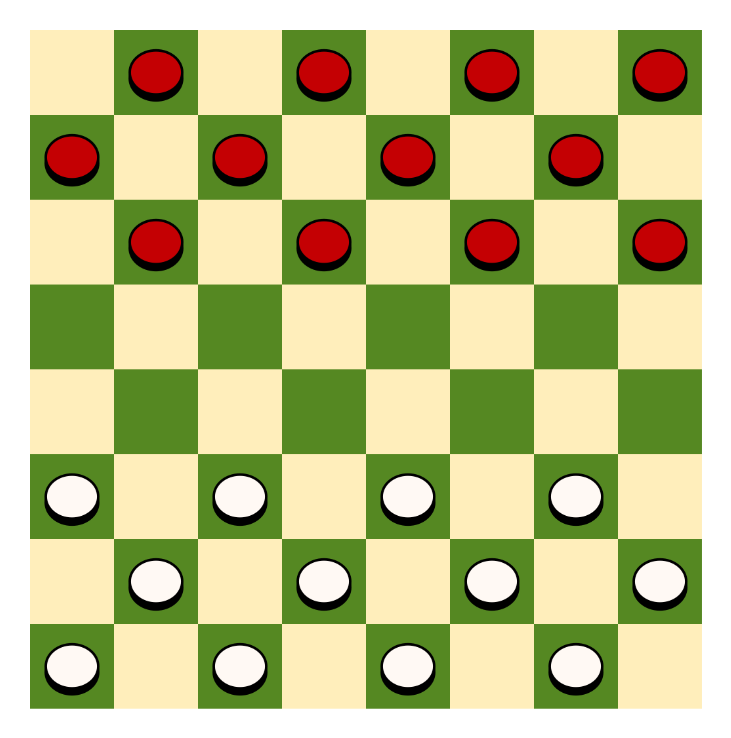
\includegraphics[scale=0.25]{checkers}
\end{frame}


\begin{frame}
	\frametitle{What is Reinforcement Learning?}
	\vspace{0.2cm}
	\begin{itemize}
		\item A machine learning paradigm focused on training agents to make sequences of decisions
		\item Key components:
		\begin{itemize}
			\item \textbf{Agent}: Learns to act in an environment
			\item \textbf{Environment}: The system with which the agent interacts
			\item  \textbf{Reward}: Feedback signal indicating the success of an action
		\end{itemize}
		\item Goal: Maximize cumulative rewards over time
	\end{itemize}
	\centering
	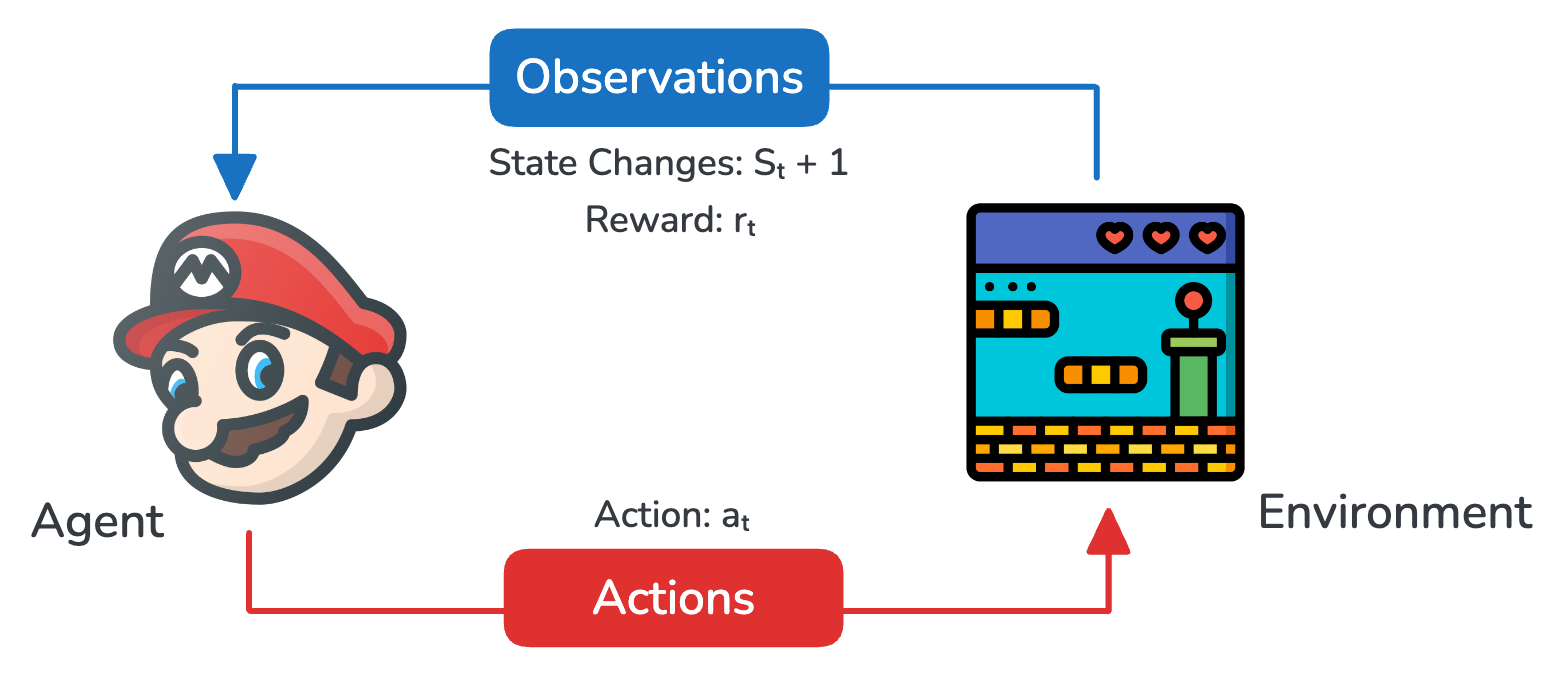
\includegraphics[scale=0.25]{rl_agent_env}
\end{frame}


% Model and algo Slides (WIP)

\begin{frame}
	\frametitle{Deep Q-Learning}
	\vspace{0.5cm}
		\begin{itemize}	
			\item reinforcement learning technique to find the optimal action-value function $Q(s,a)$
			\item It maps state-action pairs to their expected future rewards
		\end{itemize}
		 \centering
		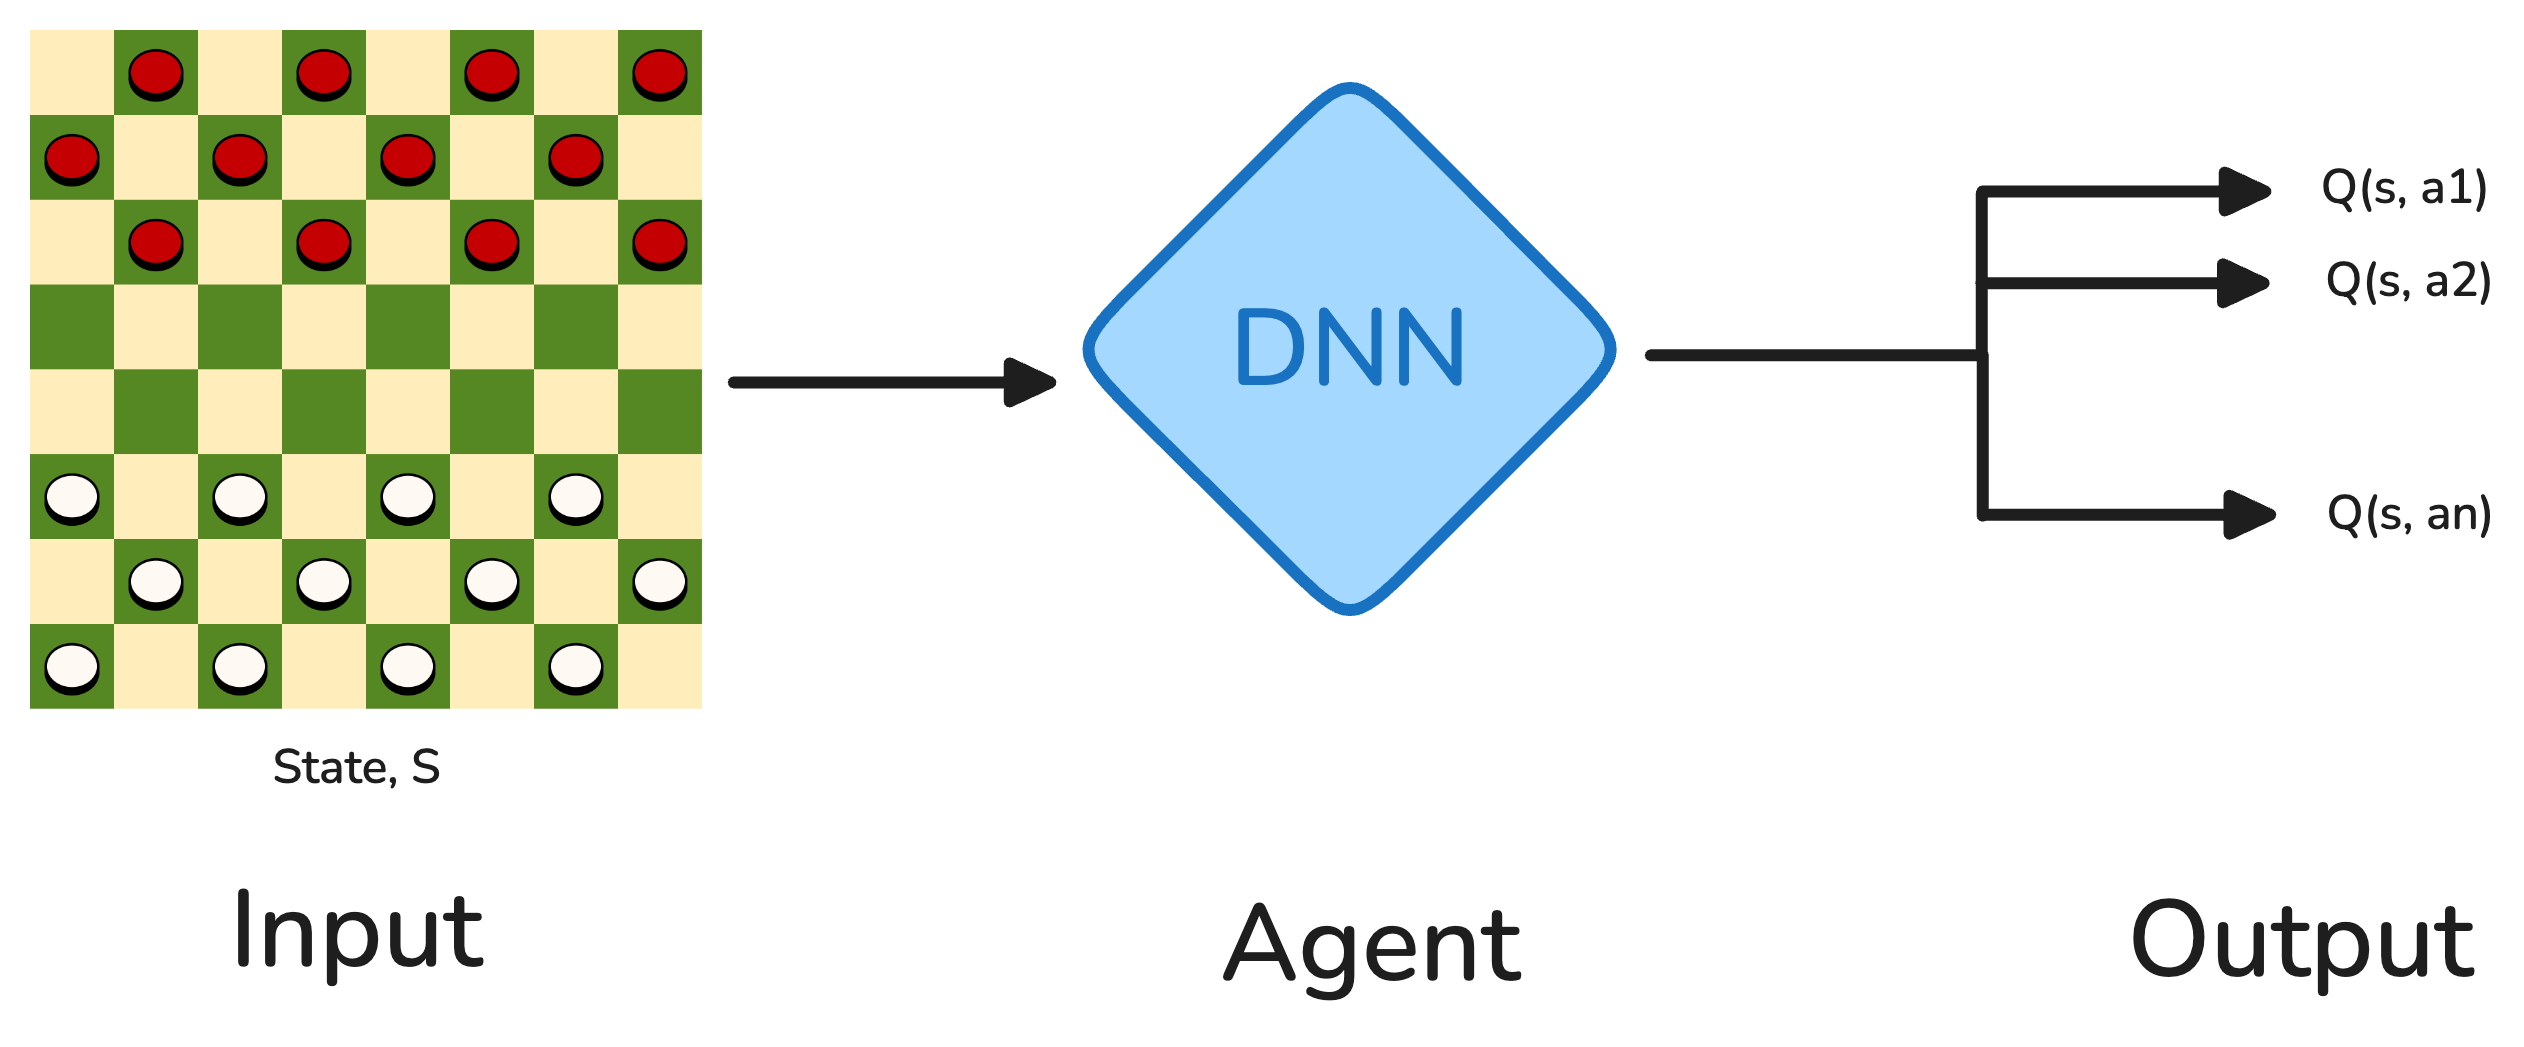
\includegraphics[scale=0.15]{dqn_checkers}
		% Q-Update rule: % $$Q(s,a) = Q(s,a) +  \alpha [r + \gamma  \ max_{a'} \ Q(s',a') - Q(s,a)]$$
			
\end{frame}

\begin{frame}
	\frametitle{Deep Q-Learning: Q-update rule}
	\vspace{1cm}
		
			
		$$Q^{\text{new}}(s_t, a_t) \leftarrow Q(s_t, a_t) 
		+ \underbrace{\alpha}_{\text{learning rate}} \cdot 
		\overbrace{\left( r_t + \underbrace{\gamma}_{\text{discount factor}} 
		\cdot \underbrace{\max_a Q(s_{t+1}, a)}_{\text{estimate of optimal future value}} 
		- \underbrace{Q(s_t, a_t)}_{\text{old value}} \right)}^{\text{temporal difference}}$$
		
		\vspace{1cm}
		\pause
		\centering
		\textbf{Challenge}: Traditional Q-learning fails for large or continuous state spaces
\end{frame}

\begin{frame}
	\frametitle{Deep Q-Learning: Solution }
	\vspace{0.5cm}
	Use a \textbf{Deep Neural Network} (DNN) as a function approximator for $Q(s,a)$ instead of a table
		\begin{itemize}		
			\item  \textbf{Input}: State $s$, \textbf{Output}: Q-values for all actions $a$
			\item \textbf{Target Network}: stabilizes training by holding fixed weights for a few updates
			\item \textbf{Experience Replay}: samples random batches of past experiences $(s,a,r,s')$ to break correlation in training data
		\end{itemize}
\end{frame}

\begin{frame}
	\frametitle{Deep Q-Learning Algorithm}
	\vspace{1cm}
	\centering
	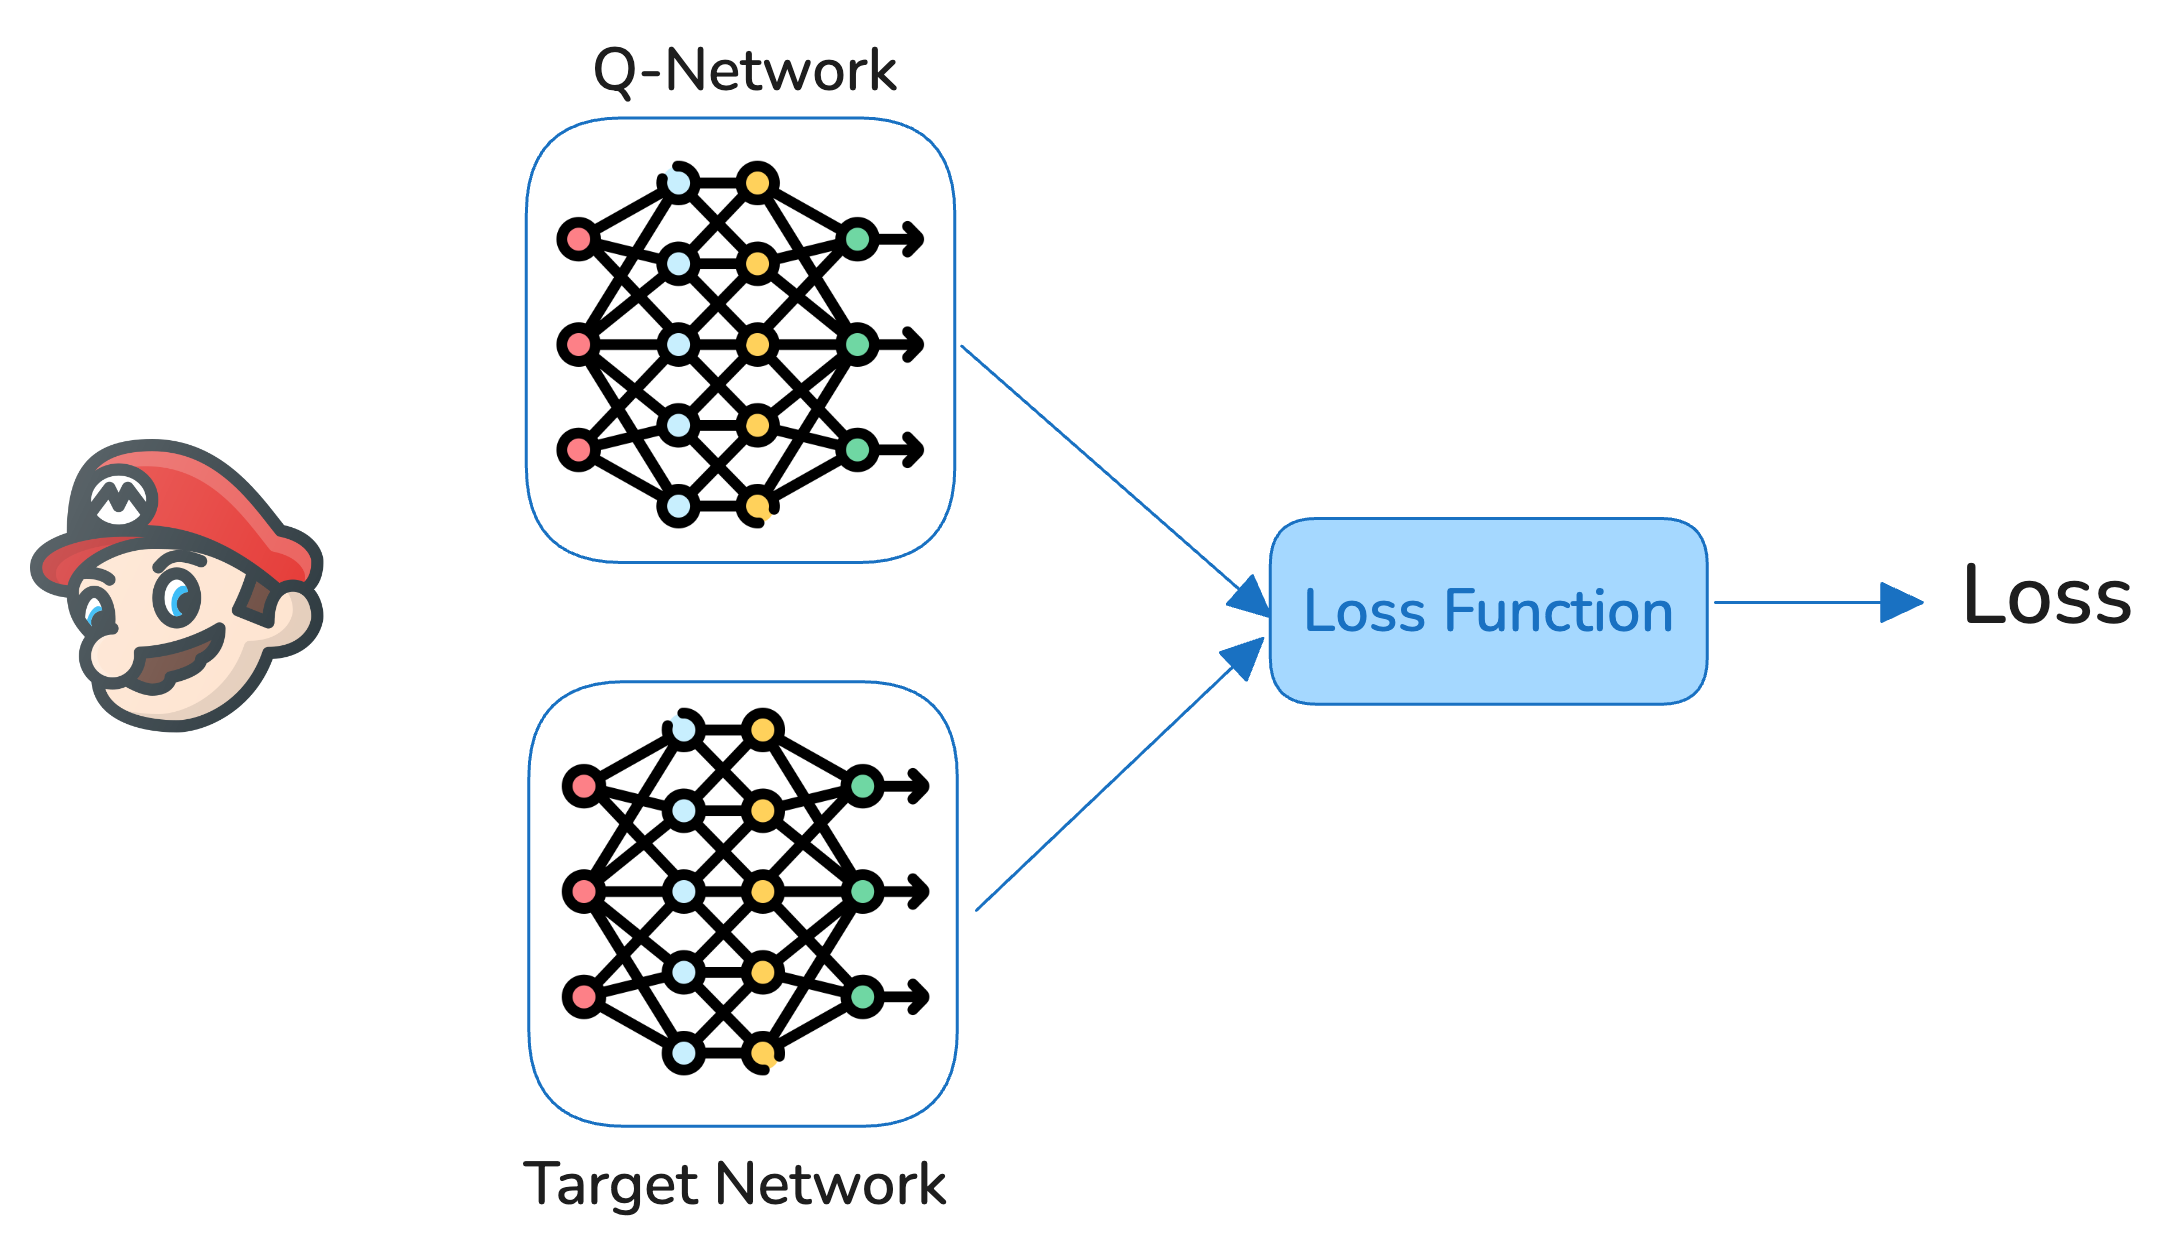
\includegraphics[scale=0.2]{lossfunction}
\end{frame}

\begin{frame}
	\frametitle{Deep Q-Learning Algorithm}
	\vspace{1cm}
	\centering
	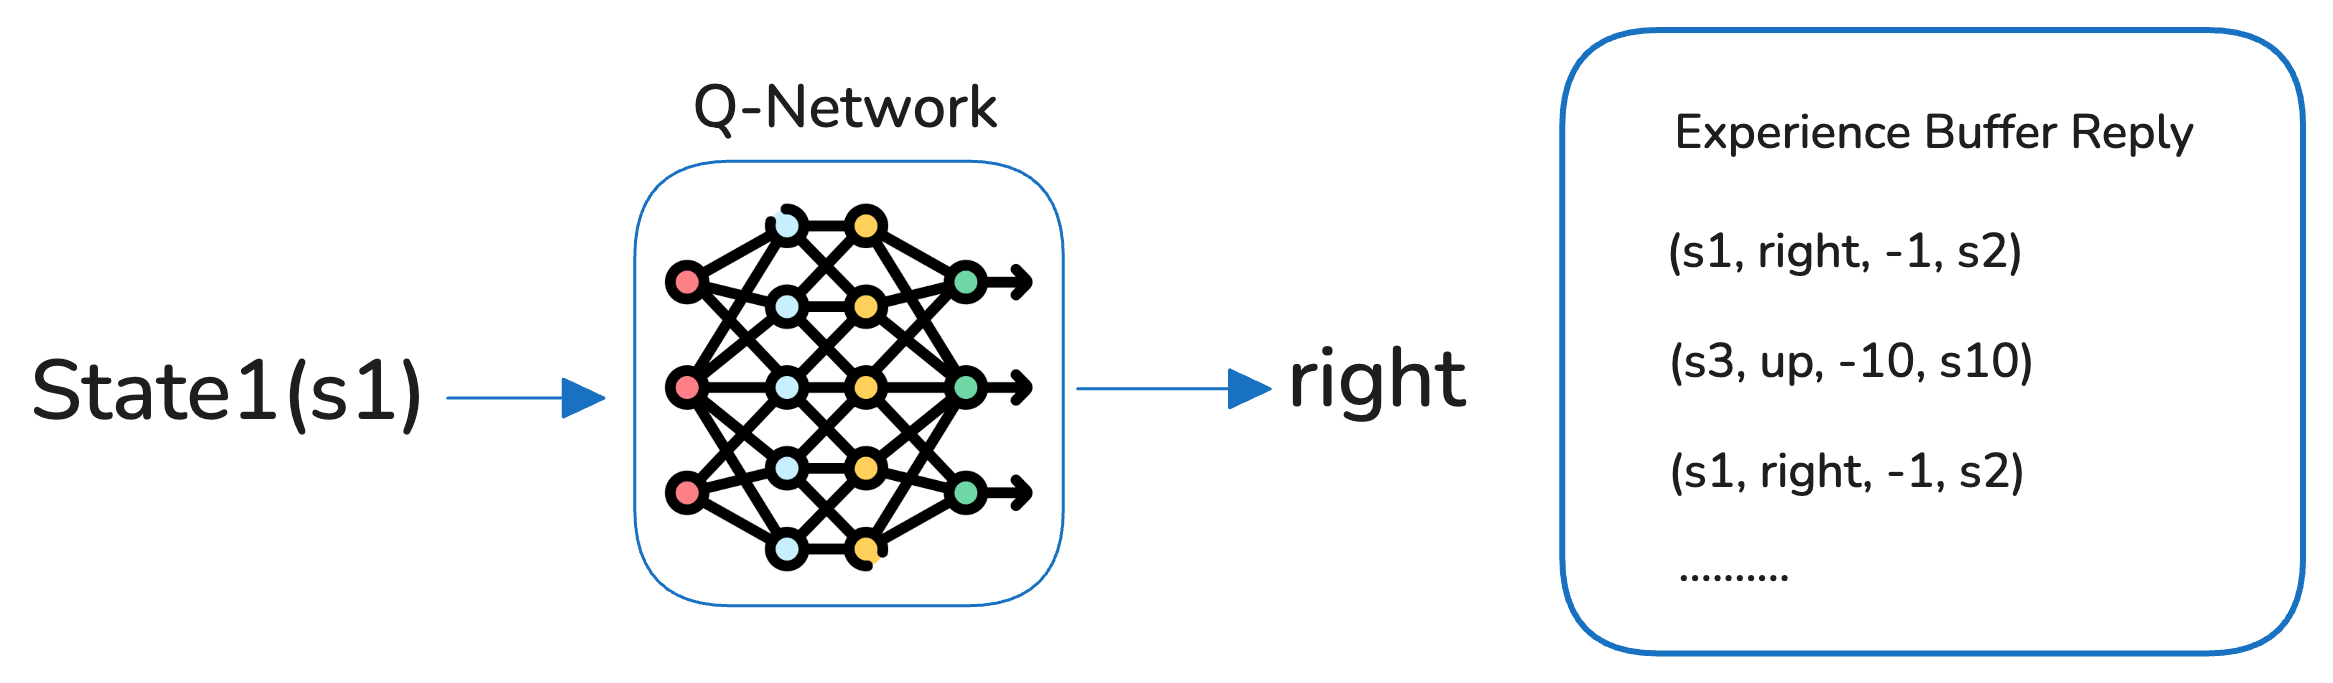
\includegraphics[scale=0.2]{buffer}
\end{frame}


\begin{frame}
	\frametitle{Deep Q-Learning Algorithm }
	\vspace{0.2cm}
	Use a \textbf{Deep Neural Network} (DNN) as a function approximator for $Q(s,a)$ instead of a table
		\begin{enumerate}		
			\pause
			\item Initialize: \\ Q-Network $Q(s,a;\theta)$ and Target Network $Q'(s,a;\theta^{-})$
			\pause
			\item Action Selection: \\ Use an $\epsilon-$ greedy policy to balance exploration vs. exploitation
			\pause
			\item Store Experience: \\ Add $(s,a,r,s')$ to a replay buffer
			\pause
			\item Train the Network: \\ 
				\begin{itemize} 
					 \item sample a minibatch from the buffer
					 \item Compute target Q-values: $y = r + \gamma \ max_{a'} \ Q'(s',a';\theta^{-})$
					\item Minimize loss: $L(\theta)=(y-Q(s,a;\theta))^2$
				\end{itemize}
			\pause
			\item Update Target Network: \\ Periodically copy weights: $\theta^{-} \leftarrow \theta$

		\end{enumerate}
\end{frame}

\begin{frame}
	\frametitle{Key Improvements and Applications}
	\vspace{0.5cm}
	Improvements:
		\begin{itemize}		
			\item \textbf{Double DQN}: Reduces overestimation of Q-values
			\item\textbf{Dueling DQN}: Separates value and advantage functions
			\item \textbf{Prioritized Experience Replay}: Samples important experiences more frequently
		\end{itemize}
	\pause
	Applications:
		\begin{itemize}
			\item Games
			\item robotics
			\item autonomous systems
		\end{itemize}
\end{frame}


% Planning and Timeline

\begin{frame}
	\frametitle{Project Planning \& Timeline}
	\vspace{0.2cm}
	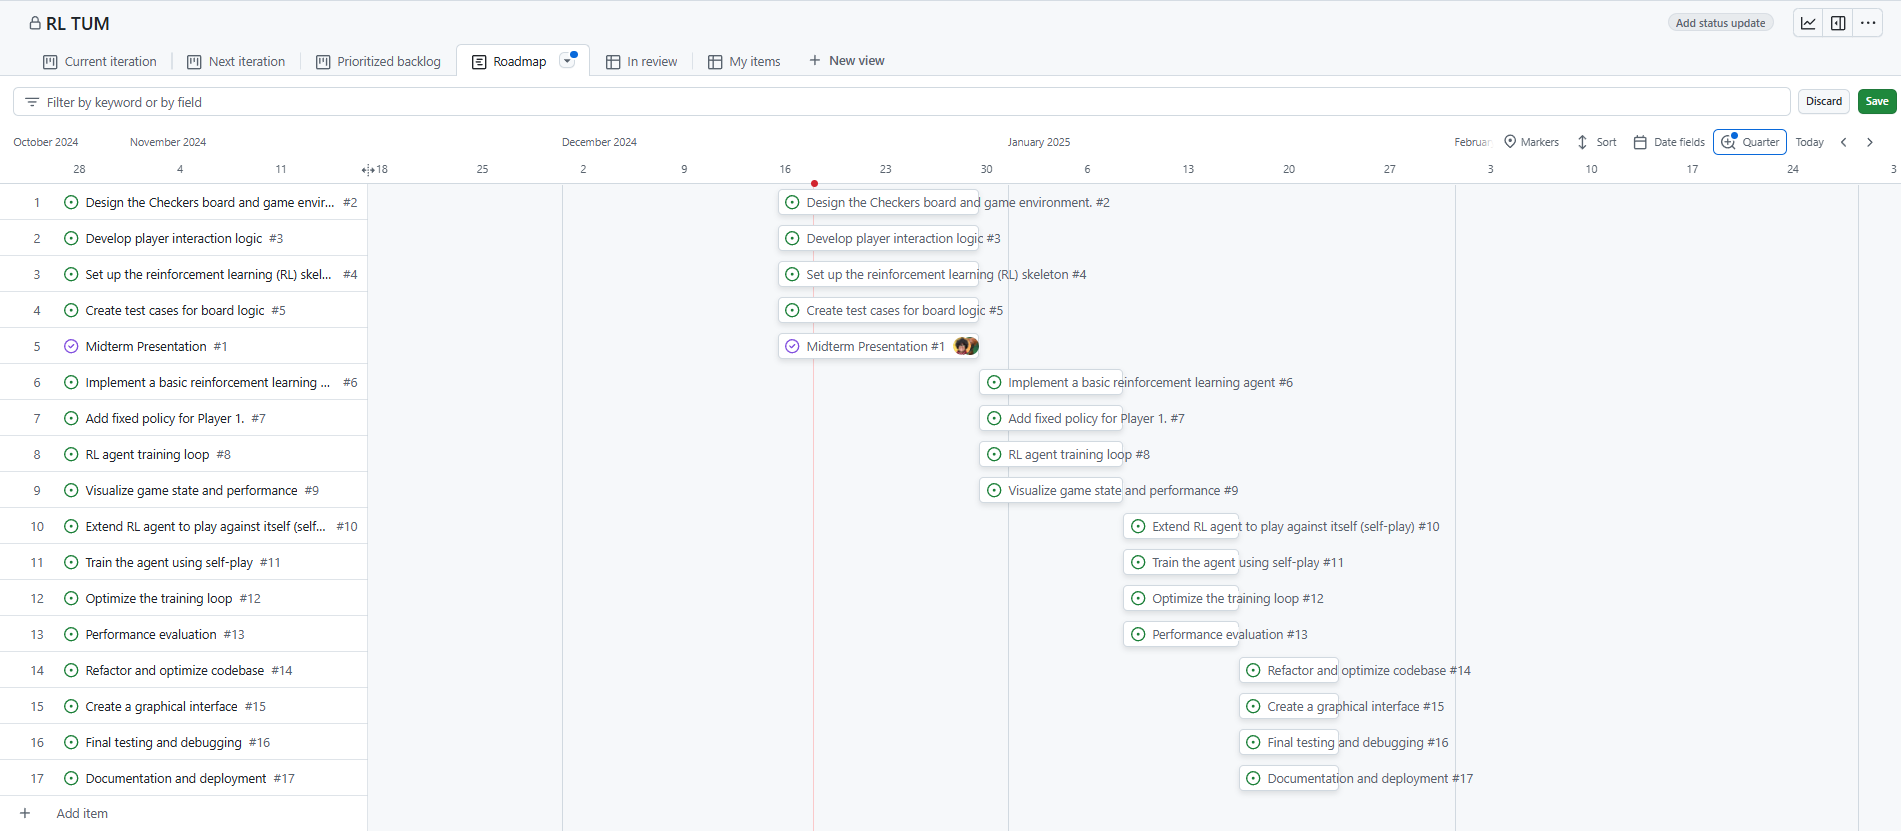
\includegraphics[scale=0.45]{project-plan}
\end{frame}

\begin{frame}
	\frametitle{Software Stack}
	\vspace{1cm}
	\begin{itemize}
		\item Python
		\item numpy (for matrix calculations)
		\item pygame (fast UI)
		\item Web frameworks
		\item tensorflow (for ML implementation)
	\end{itemize}	
\end{frame}

\begin{frame}
	\frametitle{Future Work}
	\vspace{0.5cm}
	\begin{itemize}
		\item Fine-tuning the DQN model for improved decision-making
		\item Incorporating advanced techniques like Double DQN and Dueling DQN
		\item Testing against human players to evaluate real-world performance
		\item Extending the approach to other board games or strategy games (some side-projects)
	\end{itemize}
\end{frame}


\begin{frame}
	\frametitle{Thank You}
	\vspace{1cm}
	\centering
	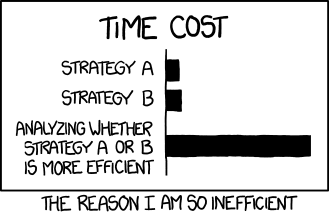
\includegraphics{efficiency} \\
	xkcd 1445
\end{frame}

% add here




%%%%%%%%%%%%%%%%%%%%%%%%%%%%%%%%%%%%%%%%%%%%%%%%%%%%%%%%%%%%%%%%%%%%%%%%%%%%%%%%
\end{document} % !!! NICHT ENTFERNEN !!!
%%%%%%%%%%%%%%%%%%%%%%%%%%%%%%%%%%%%%%%%%%%%%%%%%%%%%%%%%%%%%%%%%%%%%%%%%%%%%%%%

